% VLDB template version of 2020-08-03 enhances the ACM template, version 1.7.0:
% https://www.acm.org/publications/proceedings-template
% The ACM Latex guide provides further information about the ACM template

\documentclass[sigconf, nonacm]{acmart}

%% The following content must be adapted for the final version
% paper-specific
\newcommand\vldbdoi{XX.XX/XXX.XX}
\newcommand\vldbpages{XXX-XXX}
% issue-specific
\newcommand\vldbvolume{14}
\newcommand\vldbissue{1}
\newcommand\vldbyear{2020}
% should be fine as it is
\newcommand\vldbauthors{\authors}
\newcommand\vldbtitle{\shorttitle} 
% leave empty if no availability url should be set
\newcommand\vldbavailabilityurl{URL_TO_YOUR_ARTIFACTS}
% whether page numbers should be shown or not, use 'plain' for review versions, 'empty' for camera ready
\newcommand\vldbpagestyle{plain} 


%!TEX root = ../main.tex
\newcommand{\eat}[1]{}
\usepackage{latexsym}
\usepackage{amsfonts}
\usepackage{amsmath}
%\usepackage{amssymb}
\usepackage{color}
\usepackage{colortbl}
\usepackage{epsfig}
\usepackage{xspace}
\usepackage{graphicx}
\usepackage{subfigure}
\usepackage{pifont}
\usepackage{bm}

%\usepackage{algorithmicx}
\usepackage{xparse}

\usepackage[lined,boxed,vlined,ruled,linesnumbered]{algorithm2e}
\usepackage{algorithmicx}
\usepackage{paralist}
\usepackage{enumerate}
\usepackage{ifthen}
\usepackage{ulem}
\usepackage{makecell}

%response command
\newcommand{\stitle}[1]{\vspace{1.2ex}\noindent{\bf #1}}
\newcommand{\etitle}[1]{\vspace{0.8ex}\noindent{\underline{\textit{#1}}}}
\newcommand{\ititle}[1]{\vspace{1ex}\noindent\textbf{\textit{#1}}}
\newcommand{\overwrite}[1]{\textcolor{blue}{#1}}
\newcommand{\bfit}[1]{\textbf{\textit{#1}}}
\newcommand{\re}[1]{\noindent{\textbf{\textit{#1}}}}
%%%%%%%%%%%%%%%%%%%%%%%%%%%%%%%%%%%%%
%% DO NOT DELETE!!
%%%%%%%%%%%%%%%%%%%%%%%%%%%%%%%%%%%%%
%\usepackage{tikz}
%\usetikzlibrary{trees}

\usepackage{epsfig}
\usepackage{multirow}
\usepackage{url}

\usepackage[color,matrix,arrow,all]{xy}
%\usepackage[all,cmtip]{xy}

\usepackage{tikz}
\usetikzlibrary{shapes,snakes}
\usetikzlibrary{calc}

\newtheorem{example}{Example}
\newtheorem{theorem}{Theorem}

\newcommand{\add}[1]{\textcolor{blue}{#1}}
\newcommand{\lgl}[1]{\textcolor{blue}{#1}}
\NewDocumentCommand{\cc}{ mO{} }{\textcolor{red}{\textsuperscript{\textit{CC}}\textsf{\textbf{\small[#1]}}}}

\newcommand{\addnew}[1]{\textcolor{red}{#1}}


\NewDocumentCommand{\wjy}{ mO{} }{\textcolor{violet}{\textsuperscript{\textit{WJY}}\textsf{\textbf{\small[#1]}}}}

\NewDocumentCommand{\nan}{ mO{} }{\textcolor{blue}{\textsuperscript{\textit{dyh}}\textsf{\textbf{\small[#1]}}}}

\sloppy
\newcommand{\rtable}[1]{\ensuremath{\mathsf{#1}}}
\newcommand{\ratt}[1]{\ensuremath{\mathit{#1}}}
\newcommand{\stt}[1]{\texttt{\small{#1}}}
\newcommand{\at}[1]{\protect\ensuremath{\mathsf{#1}}\xspace}
\newcommand{\myhrule}{\rule[.5pt]{\hsize}{.5pt}}
\newcommand{\oneurl}[1]{\texttt{#1}}
\newcommand{\tabstrut}{\rule{0pt}{4pt}\vspace{-0.1in}}
\newcommand{\stab}{\vspace{1.2ex}\noindent}
\newcommand{\sstab}{\rule{0pt}{8pt}\\[-2.2ex]}
\newcommand{\vs}{\vspace{1ex}}
\newcommand{\exa}[2]{{\tt\begin{tabbing}\hspace{#1}\=\+\kill #2\end{tabbing}}}
\newcommand{\ra}{\rightarrow}
\newcommand{\match}{\rightleftharpoons}


\newcommand{\sys}{\texttt{MisDetect}\xspace}



\newcommand{\la}{\leftarrow}
\newcommand{\bi}{\begin{itemize}}
	\newcommand{\ei}{\end{itemize}}
\newcommand{\mat}[2]{{\begin{tabbing}\hspace{#1}\=\+\kill #2\end{tabbing}}}
\newcommand{\be}{\begin{enumerate}}
	\newcommand{\ee}{\end{enumerate}}
\newcommand{\beqn}{\begin{eqnarray*}}
	\newcommand{\eeqn}{\end{eqnarray*}}

\newcommand{\ie}{$i.e.$,\xspace}
\newcommand{\eg}{$e.g.$,\xspace}
\newcommand{\wrt}{w.r.t.\xspace}
\newcommand{\aka}{a.k.a.\xspace}
\newcommand{\kwlog}{\emph{w.l.o.g.}\xspace}

\newcommand{\eop}{\hspace*{\fill}\mbox{$\Box$}\vspace{1ex}}     % End of proof

\makeatletter
\newcommand\figcaption{\def\@captype{figure}\caption}
\newcommand\tabcaption{\def\@captype{table}\caption}
\makeatother

\newcommand{\reminder}[1]{ {\mbox{$<==$}} [[[ \bluefont{ \bf #1 } ]]] {\mbox{$==>$}}}

\definecolor{shadecolor}{RGB}{220,220,220}
\newcommand{\mybox}[1]{\vspace{1.5ex}\par\noindent\colorbox{shadecolor}
	{\parbox{\dimexpr\columnwidth-2\fboxsep\relax}{#1}}\vspace{1ex}}


\tikzstyle{mybox} = [draw=black, fill=black!5, thick,
rectangle, rounded corners, inner sep=0pt, inner ysep=2pt]
\tikzstyle{fancytitle} =[fill=black, text=white]











\begin{document}
\title{Synthetic Data Generation for Machine Learning Models }

%%
%% The "author" command and its associated commands are used to define the authors and their affiliations.
\author{Ben Trovato}
\affiliation{%
  \institution{Institute for Clarity in Documentation}
  \streetaddress{P.O. Box 1212}
  \city{Dublin}
  \state{Ireland}
  \postcode{43017-6221}
}
\email{trovato@corporation.com}



%%
%% The abstract is a short summary of the work to be presented in the
%% article.
\begin{abstract}
Abstract here.
\end{abstract}

\maketitle

%%% do not modify the following VLDB block %%
%%% VLDB block start %%%
\pagestyle{\vldbpagestyle}
\begingroup\small\noindent\raggedright\textbf{PVLDB Reference Format:}\\
\vldbauthors. \vldbtitle. PVLDB, \vldbvolume(\vldbissue): \vldbpages, \vldbyear.\\
\href{https://doi.org/\vldbdoi}{doi:\vldbdoi}
\endgroup
\begingroup
\renewcommand\thefootnote{}\footnote{\noindent
This work is licensed under the Creative Commons BY-NC-ND 4.0 International License. Visit \url{https://creativecommons.org/licenses/by-nc-nd/4.0/} to view a copy of this license. For any use beyond those covered by this license, obtain permission by emailing \href{mailto:info@vldb.org}{info@vldb.org}. Copyright is held by the owner/author(s). Publication rights licensed to the VLDB Endowment. \\
\raggedright Proceedings of the VLDB Endowment, Vol. \vldbvolume, No. \vldbissue\ %
ISSN 2150-8097. \\
\href{https://doi.org/\vldbdoi}{doi:\vldbdoi} \\
}\addtocounter{footnote}{-1}\endgroup
%%% VLDB block end %%%

%%% do not modify the following VLDB block %%
%%% VLDB block start %%%
\ifdefempty{\vldbavailabilityurl}{}{
\vspace{.3cm}
\begingroup\small\noindent\raggedright\textbf{PVLDB Artifact Availability:}\\
The source code, data, and/or other artifacts have been made available at \url{\vldbavailabilityurl}.
\endgroup
}
%%% VLDB block end %%%




%!TEX root = ../main.tex
\section{Introduction} 
\label{sec:intro}
Data quality is one of the most significant problems in data management, among which mislabels are a common dirty data type that could directly lead to  low-quality data analysis  and misleading business decisions. Labels are always large-scale and error-prone because they may be crowdsourced from non-experts or collected from web annotations, so it is inevitable to use automatic methods to detect mislabels. However, existing mislabel detection approaches suffer from fair accuracy.


\stitle{Existing Solutions.} Traditional methods~\cite{} rely on the data locality to detect mislabels. For example, in order to whether the label of an instance in a dataset is correct, the typical KNN method~\cite{} checks its neighbors, and if they have inconsistent labels, the instance tends to be mislabeled, otherwise it is a clean one. This type of methods has low detection accuracy because they just consider the local neighbors of each instance rather than the entire dataset. Therefore, to improve the accuracy, machine learning (ML) models are incorporated to help mislabel detection~\cite{} because intuitively,  mislabels definitely have impact on the supervised model training. For instances, ensemble-based methods~\cite{} involve multiple models to train on the entire dataset and check the consistency of the prediction results from these models for each instance. Cleanlab~\cite{} utilizes confident learning to estimate the joint distribution of mislabels and correct labels. This line of methods can capture the entire data distribution of the dataset through ML and avoid the data locality problem. However, the accuracy is still not high because they learn the distribution from both the incorrect and correct labels. In this way the model has already fitted on the dirty data, and thus the learned distribution is not accurate, leading to inaccurate prediction results.


\stitle{Challenge.} As discussed above, to pursue high accuracy of mislabel detection, we have to consider the data distribution of the entire dataset, but the main challenge is that how to alleviate the impact of mislabels on the learned distribution.

%\stitle{Problem.}
%Our main research question in this paper is how to \textit{detect mislabeled data in the large training set which will be used for the downstream meachine learning model} and filter it to improve the data quality of training set. A positive answer to this question is crucial as it can help machine learning model to learn more correctly about the distribution of the training set, so as to obtain better model performance.


\stitle{Observation.} 

\stitle{Our proposal.}
Our main idea is to find out the instance in the training set which is labeled incorrectly.
More specifically, \nan{Add more details later.}

\stitle{Contributions.}
Our contributions are summarized as follows:


\begin{figure*}
	\centering
	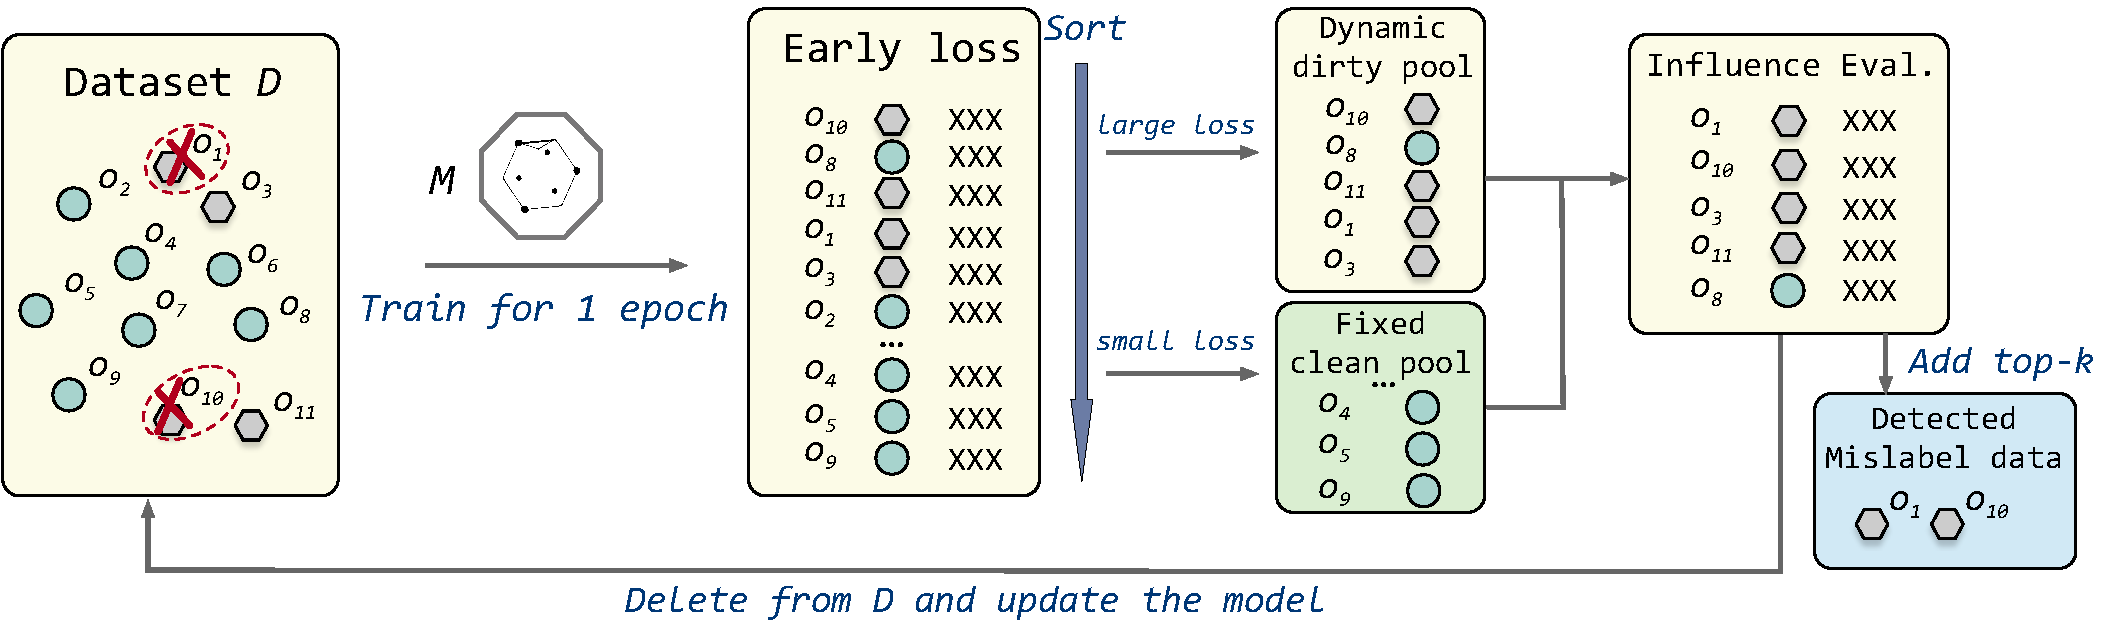
\includegraphics[width=\textwidth]{figures/framework}
	\caption{\sys Framework}
	\label{fig:framework}
\end{figure*}


\be
	\item 
	\item 
	\item \nan{If we can have a good summary of experiments, we can either add here or use a ``stitle'' section to highlight the empirical findings.}
\ee



% \begin{figure*}
%	\centering
%	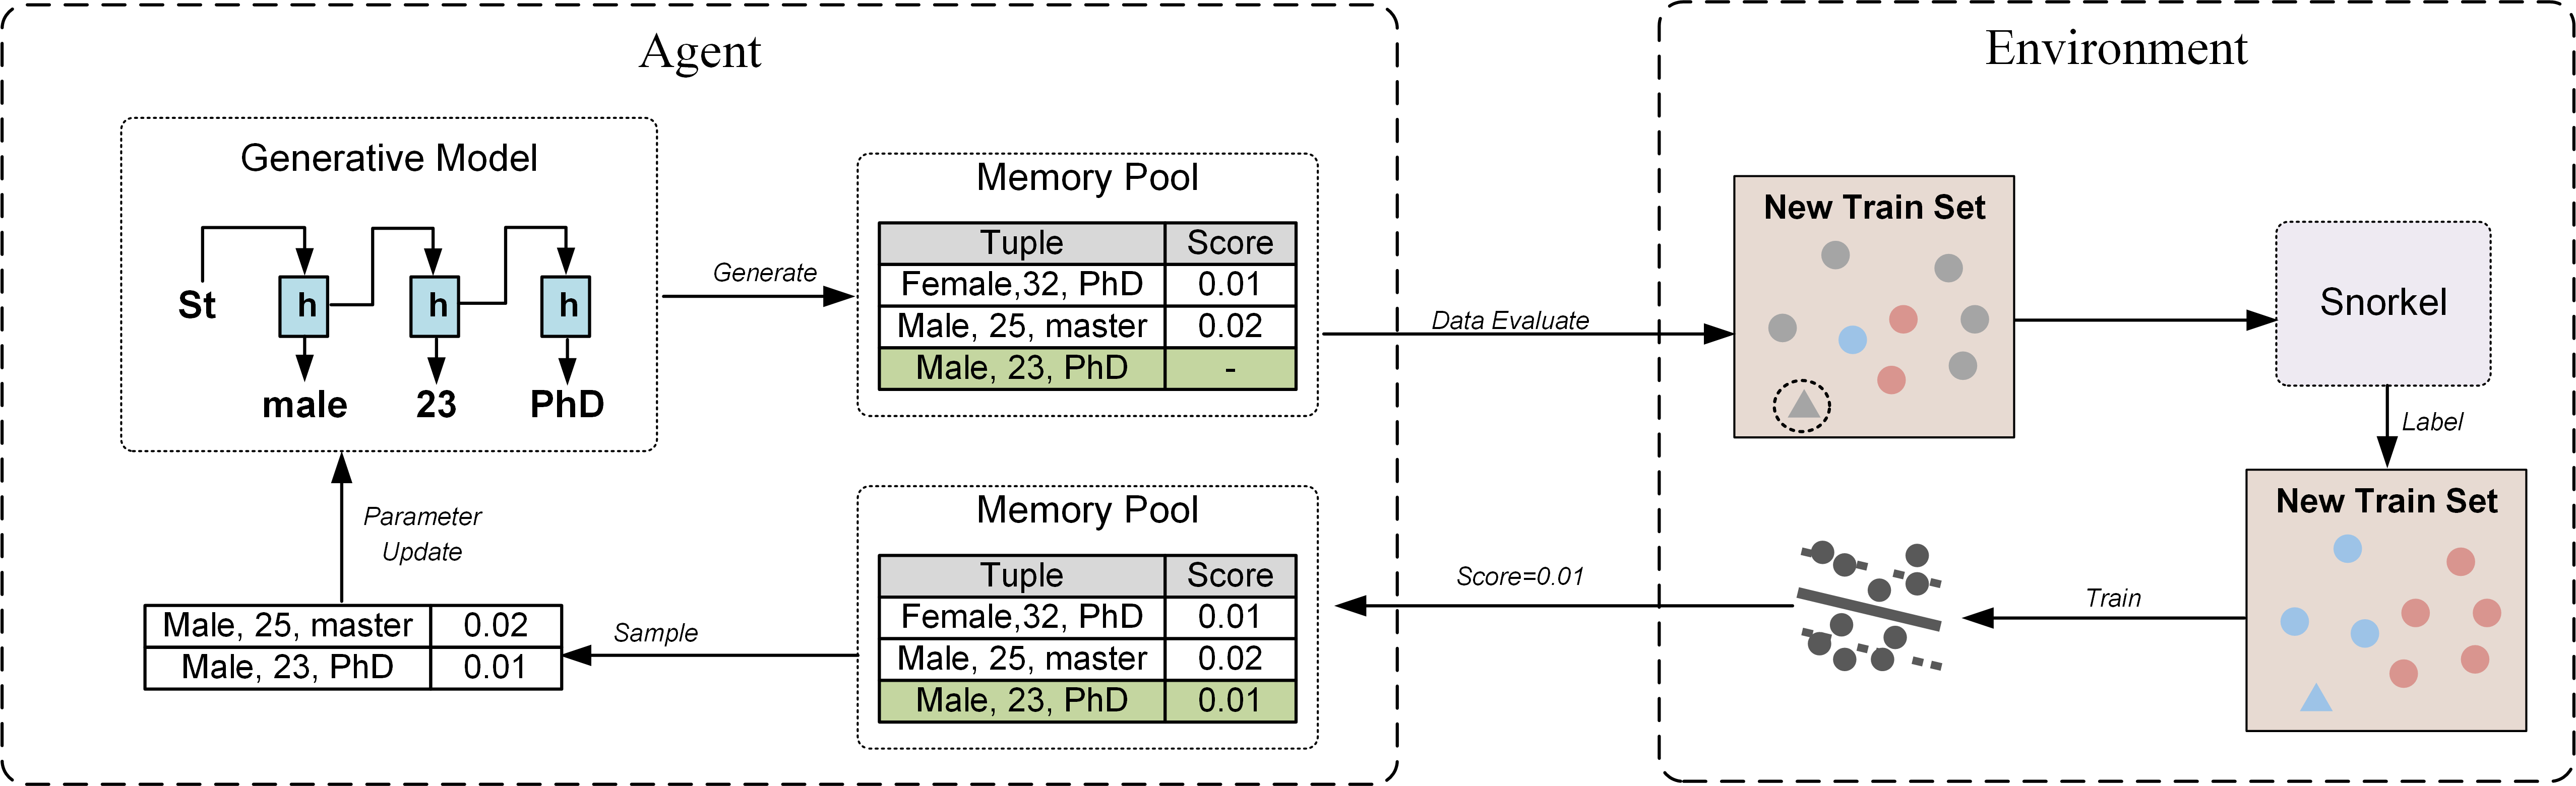
\includegraphics[width=\textwidth]{figures/overview.png}
%	\caption{Framework}
%	\label{fig:framework}
% \end{figure*}

% \begin{itemize}
% 	\item The difference between traditional data generation and ours (for ML model).
% 	\item (Challenge) The key challenges of this problem: learn the generative model from feedback; how to evaluate generated tuples.
% \end{itemize}
%!TEX root = ../main.tex
\section{Preliminary} 
\label{sec:pre}

\subsection{Problem Statement}

\stitle{Machine learning task.}

The setting of our problems.

Input:
\begin{itemize}
	\item A small training set with lots of unlabeled data
	\item A validation (test) set
	\item A user-specified downstream model
\end{itemize}

Output: A trained downstream model with best performance on the test set.


\subsection{Deep Generative Models for Tables}


\subsection{Reinforcement Learning: A Primer}



\nan{We should give some background about generative models and RL -- not sure how many reviewers know these in details.}
%!TEX root = ../main.tex
\section{Framework} 
\label{sec:framework}

To address the above challenges, we design the \sys framework that introduces the early loss to well distinguish mislabeled instances from clean ones. As shown in Figure~\ref{fig:framework}, the basic idea of \sys is that with the number of epochs increases from the beginning, at early epochs, we can regard a number of  instances with small loss as clean instances, over which we  can train a model almost without  dirty data information. Then we can leverage the parameter of this model as a replacement of $w^*$. Meanwhile, we can also let a number of  instances with large  loss constitute  a pool of mislabeled instance candidates, among which we pick some  instances with high influence based on $w^*$. Afterwards, we identify these instances as mislabeled and remove them, leading to more accurate mislabel detection for further epochs. 

\stitle{Early loss based detection.} As discussed in Section~\ref{sec:intro},  mislabeled instances tend to have a large early loss because the model is hard to fit them, especially at early training stages. In Figure~\ref{fig:framework}, we can see that we detect mislabels iteratively  as the training progresses.
Specifically, at the  $j$-th  epoch,  we define the loss of the $i$-th instance  as  $l_i^j = y_i - w_j\cdot x_i$, where $w_j$ is the model parameter of this epoch. Then we include a proportion of instances with  large loss as the candidate pool of mislabeled instances, denoted by $\dirtypool$, because they are likely to be dirty. Similarly, the instances with small loss are very likely to be clean because they can be well fitted by the model at early epochs.  Therefore, we construct another  pool $\cleanpool$ of clean  instances, over which we train a model to measure the influences of instances in $\dirtypool$. This will be briefly introduced next. Note that we fix  $\cleanpool$ after the first epoch because these instances that have already been fitted with small loss will not vary much afterwards, so  we do not have to iteratively update it considering the efficiency. However, $\dirtypool$ has to be dynamically updated since the loss is likely to vary when it is large at the beginning.


 %Then, for  $L_j = \{l_i^j| i\in[1,N]\}$, we can compute the standard deviation $\sigma_j = \sqrt{\frac{\sum_{i=1}^{N}(l_i^j-\mu_j)^2}{N}}$, where $\mu_j$ is the average of $L_j$. 
\stitle{Influence evaluation.} Given $\dirtypool$, a straightforward method is to   just directly remove all instances in it or someones with the largest loss, but although the removed instances tend to be mislabeled, they may not influence the current model much. Recap that in Equation~\ref{eqa:optimize},  we aim to remove mislabeled instances such that  the model can be close to $w^*$. And the more quickly (with fewer epochs) we approach  $w^*$, the easier for the model to detect mislabels because $w^*$ is the ideal parameter  trained over all clean instances. 

Since we cannot know  $w^*$ in advance, in order to measure the influence of removing each instance on approaching  $w^*$, a basic solution is to instead measure the influence of removing the instance on the model trained with current dataset. Although we can compute this influence efficiently without retraining using the influence function~\cite{}, it does not perform well. The reason is that  such strategy cannot provide evident signal because current dataset is mixed with dirty and clean instances, and thus no matter how large the influence of the instance in fact is, the  result  calculated by the influence function is not obvious.

Therefore, we propose a new influence computation method customized to our problem. As introduced before, based on the early loss,  we construct a clean pool $\cleanpool$, in which the instances are very confidently clean. We train a model $M_c$ with parameter $w_c$ over $\cleanpool$. For each instance $o_i$, we measure its influence of adding $o_i$ to $\cleanpool$. Since $\cleanpool$ is clean, adding a dirty instance will be much more sensitive than the aforementioned method.
Intuitively, if an instance has a large impact on a model after adding it into the dataset  $w.r.t.$  $w_c$, removing it will be rather helpful  for   quickly  approaching $w^*$ because $w_c$ can be regarded as an approximation of $w^*$. We will introduce this in detail in Section~\ref{sec:influence}.




\stitle{False positive elimination.} During the process of mislabel detection, there inevitably exist some false positive instances, \ie  they are in fact clean but are identified as mislabeled ones. One main reason is that there exist some outliers in $\train$, which will also produce large loss at early stages of training. To address this, we propose to detect outliers before training, and temporarily put them on hold without participating in mislabel detection during training. In this way, these outliers will not be identified as false positives although they have large loss. When the mislabel detection process terminates, we can leverage the mislabeled/clean instances that have already been detected to check which ones among these outliers are mislabeled.

On the other hand, there will also be some clean instances that are not classified as outliers, but they could produce large loss as they are hard to fit for a model. We also expect to identify these false positives. In practice, we observe that  they are harder to fit than most clean instances, butx still easier  than those mislabeled ones, so we propose to address this problem by tracking the variation of loss. Intuitively, if the loss  of an instance with initial large loss quickly decreases, it tends to be a false positive. Otherwise, we still keep it as a mislabeled instance. We will discuss how to eliminate false positives in detail in Section~\ref{sec:fp}.

\cc{Current figure does not show false positive elimination.}

\stitle{Overall \sys Framework.} To summarize, given a train set $\train$, we first identify a subset of  outliers $\outlier$ in it and temporarily remove these outliers from $\train$ (\ie $\train = \train/ \outlier$).
\cc{Next, an important step is to estimate the number of mislabeled instances in $\train$ such that we can decide when to stop the detection process (Section~\ref{sec:loss}).}
 Afterwards, we iterative train over $\train$ and detect mislabeled instances in each epoch, as shown in Figure~\ref{fig:framework}. At each epoch, we can obtain the loss of each instance. Then, we will extract the top largest ones to constitute $\dirtypool$, and the bottom  smallest ones to constitute $\cleanpool$. On the basis of $\cleanpool$, we can well evaluate the influence of each instance in $\dirtypool$ and select the top-$k$ instances with high influence as mislabeled ones. For example, at current epoch in Figure~\ref{fig:framework}, $\dirtypool$ consists of $o_{10}, o_{8}, o_{11}, o_{1}, o_{3}$. Next, we evaluate the influence. Although $o_{8}$ is a clean instance with a large loss, its influence is not large if we put it into $\cleanpool$ that is full of clean instances. Hence, $o_{8}$ will not be detected in this epoch, and $o_{1},o_{10}$ with high influence will be detected and removed. Then, another epoch starts, and this repeats until we have detected the number of estimated mislabels. Note that during the training process, we will also track the loss variation of each instance to identify some candidates that we suspect they are false positives.
 Finally, we will look back to these suspicious candidates as well as  $\outlier$ to check whether they are mislabeled to further improve the detection accuracy.




%\nan{I found that many reviewers will complain that (1) the above figure is too complicated to understand, and (2) the explanation of the figure is not clear. If the reviewers can fully understand and appreciate this framework figure and we have good empirical results, it is more than 50\% done.}

%\subsection{System Overview}

% \begin{itemize}
% 	\item (Motivation) Why use RL to solve the data generation problem.
% 	\item How to use RL to solve this problem.
% 	\item The workflow of the system, \ie the interaction between agent and environment.
% \end{itemize}

%!TEX root = ../main.tex
\section{Synthetic Data Generation} 
\label{sec:datagen}

\nan{This section should be only about data generation, no need to discuss RL, but we need to justify why we choose LSTM, not other models such as VAEs or diffusion models.}

\begin{itemize}
	\item (State) How to encode the features, \ie categorical feature and numerical data.
	\item (Action) The output of the generative model.
	\item (Model design) The RNN model.
	\item How to train the RNN model, \ie the Actor-Critic framework.
\end{itemize}





%!TEX root = ../main.tex
\section{Data Evaluation} 
\label{sec:dataeva}

\nan{This section should discuss the design of the RL part.}

\begin{itemize}
	\item Reward computation: how to compute the score for one tuple.
	\item How to use snorkel to label the data.
	\item Probabilistic label and downstream model training.
\end{itemize}


\section{System XXX}

\nan{We should give a name of the system \sys?}

\nan{You can give an algorithm pseudocode here, about how to stitch Section 4 and Section 5 together, which must be consistent with the framework figure in Section 3.}
%!TEX root = ../main.tex
\section{Experiment} 
\label{sec:exp}

\subsection{Experimental Settings}

\textbf{\textit{\underline{Dataset.}}}We evalute our algorithm on 7 different real-world datasets from a diverse array of domains, whose size varying from the magnitude of $10^{3}$ to $10^{6}$ and the number of class differ from 2 to 100. We first used the dataset form CleanML, which have been performed synthetic mislabel injection with the strategy that flipping 5\% of the labels in each class. Then, we also use different kinds of dataset including image and table and dataset with large number of classes to further verify the effectiveness and scalability of our algorithm. The details are listed as follows:

\be
\item USCensus: This dataset contains 32,561 items about US Census records for adults. Each item has 14 attributes, such as age, education, sex, etc. The classification goal is to predict whether the adult earns more than \$50,000.
\item Marketing: A total of 8993 records are contained in this dataset, which information about household income including education, sex. etc. The goal is to make predictions about whether the annual family income is less than \$25,000. 
\item EEG: This dataset consists of 14,980 Electroencephalogram recordings with 14 Electroencephalogram attributes varying from AF3 to, AF4 The classification task is to predict whether the eye-state is closed or open. 
\item CIFAR-10: The dataset is a computer vision data set for universal object recognition, which contains 50000 32 X 32 RGB color pictures, a total of 10 categories. The task is to predict which kind does the picture belong to. Mislabeled data are artificially introduced by flipping labels of 40\% for each type of the dataset randomly. \textbf{(need explain?)}
\item CIFAR-100: This dataset is like CIFAR-10, except that it has a total of 100 classes, and each class contains 500 images. The classification task is also to predict the category of a given picture.
\item CovType: This is also a muti-classification dataset, which contains 7 different forest cover type. With a total of 581012 samples, and each sample consist of 54 attributes, such as Elevation, Wilderness Area, Horizontal Distance To Roadway etc.
\item Mobile Price Prediction: This is a small tabular dataset with only 2000 records. The task is to predict price range of the mobile on the basis of the information about the mobile, specification like Battery power, 3G enabled , wifi ,Bluetooth, Ram etc.\textbf{(need remove?)}
%\item \nan{If we can have a good summary of experiments, we can either add here or use a ``stitle'' section to highlight the empirical findings.}
\ee
\textbf{\textit{\underline{Method.}}}We compare our approach against several competing mislabel detection methods. First, we consider 10 baselines:

1. \textbf{K-Nearest Neighbor(KNN):} The method counts the number of inconsistencies between the label of a training instance and the labels of its surrounding neighbors. If there is strong evidence of distinction among the labels, the training instance is marked as mislabeled. This kind of method is called local learning method.

2. \textbf{Nearest Centroid Neighborhood (NCN):} This method is also belong to local learning method, which assumes that the labels of mislabeled instances tend to disagree with the labels of other instances in their surrounding neighborhood. The difference between KNN and this method is the approach about how to find the nearest neighbor.

3. \textbf{Training Set Debugging Using Trusted Items(DUTI):} DUTI utilizes a small set of additional "trusted items"to help detect incorrectly labeled item, which core is to finds the smallest changes for the labels in training set such that the classifier trained on the changed dataset classify all the trusted items correctly. DUTI proposes an iterative algorithm to achieve its goal.

4. \textbf{Forgetting Events:} In the process of model training, a sample has been correctly classified by the model. With the update of model parameters, the sample has been incorrectly classified. This process is called a forgetting event of the sample. This method identifies a mislabel sample based on one assumption that noisy sample often experience more forgetting events than normal samples during model training. 

5. \textbf{Ensemble-based method with consensus filter:}  Ensemble-based method assumes that multiple, independent clissifiers often result in conflicting labels about incorrectly labeled training sample. Algorithms that belong to this category vary in terms of how the different classifiers are constructed. Besides, the consensus filter is a strategy which means that a training example could be marked as a mislabel data only if it is misclassified by all the classifiers in the ensemble.

6. \textbf{Ensemble-based method with majority vote:}  The main idea of this method is tha same as the Ensemble-based method with consensus filter.The only inconsistency between them is that majority vote strategy considers an example to be mislabeled if it disagrees with the majority vote of the classifiers.

7. \textbf{Cleanlab:} Cleanlab proposes an emerging framework called confident learning, which core for detection include two main steps: Count and Clean. The first step is to estimate a joint distribution directly between incorrectly labeled data and uncorrupted(real) data based on the assumption of classification noise process(CNP)[]. After that, some instances in the training set would be tabbed as mislabel based on the joint distribution matrix computed above in the second step.

8. \textbf{Noisy Cross-Validation(NCV):} This method first randomly devides a noisy training set into two halves, then train a neural network for these two half separately. After that, the network which is trained on one half will be applied to another half of the dataset. A sample would be identified as mislabel when its current label is different from its predicted label.

9. \textbf{Iterative Noisy Cross-Validation(INCV):} Obviously, this is a iterative method about noisy cross-validation. Apart from selecting mislabel samples, the INCV removes samples that have large categorical cross entropy loss at each iteration.

10. \textbf{Partition Filter:} This method partitions a noisy dataset into multi-subsets, and then construct a good classifier from each subset iterately. For a given training sample, all classifier will be applied on it, the mislabel sample often have higher probability to have larger misclassified times.

We also consider three variants of our algorithm. The goal is to compare the effectiveness of the cross-validation using both early loss and parameter influence. For all variations, we use the same training paradigms. We consider the following variants:

1. \textbf{MisDetect Without Iteration: } This variant just does the detection once, which means choicing a very big dirty pool containing instances with large early loss and a clean pool to test the influence of each instance, then directly filter all the mislabel instances with large influence in the dirty pool without iteration.

2. \textbf{MisDetect Without Parameter Influence:} Apparently, this variant does not test the parameter influence after dirty pool is established at each iteration. It just consider the loss of each instance at initial training stage.

3. \textbf{MisDetect Without Early Loss:} This variant using parameter influence as the main detect method, in other words, it does not consider the loss of every instance in the training set except needing a clean pool which is created through early loss, the instance with large influence will be detected as mislabel data in this variant.

\textbf{\textit{\underline{Hyper-prameter Setting.}}} We train convolution neural network for image-classification task and simple 3-layers perceptron for tabular dataset.Both networks apply learning rate with 0.001 and optimizer with Adam. For CIFAR-10, CIFAR-100, CovType and Mobile Price Prediction datasets, we inject mislabel data by flipping labels of 20\% for each type of the dataset randomly. For MisDetect, we chose XXX as the clean pool len.For Ensemble-based method, we use a toal of 10 different models,such as AdaBoost, RandomForest, Support Vector Machine, etc. For Cleanlab, we use LogisticRegression to compute the thresholds for noisy estimation.\textbf{(need?)}

\textbf{\textit{\underline{Evaluation Metrics.}}}We mainly focus on the effectiveness of our algorithm and other baselines, so we take precision, recall and F1-score as the most important metrics.

\subsection{Comparison with Baselines}

Given that MisDetect is a iterative detection method,

\subsection{Mislabel Ratio Evaluation}

\subsection{Mislabel Distribution Evaluation}

We test the algorithms on two types of label noise: symmetric and class-conditional label noise. In symmetric label noise, each label is randomly flipped to any of the remaining classes with equal probability, whereas for class-conditional noise, label flipping is done in a set of similar classes. For example, 

\subsection{Model Evaluation}

\subsection{Stop Condition Evaluation}

%!TEX root = ../main.tex
\section{Related Work} 
\label{sec:related}

%!TEX root = ../main.tex
\section{Conclusion} 
\label{sec:con}







%\begin{acks}
% This work was supported by the [...] Research Fund of [...] (Number [...]). Additional funding was provided by [...] and [...]. We also thank [...] for contributing [...].
%\end{acks}

%\clearpage

\normalem
\bibliographystyle{ACM-Reference-Format}
\bibliography{bib/ref}

\end{document}
\endinput
